\documentclass[11pt]{article}

\usepackage{enumerate}

\usepackage{fullpage}
\usepackage{framed}
\usepackage[numbers]{natbib}
\usepackage{dsfont}
\usepackage{latexsym}
\usepackage{amsmath}
\usepackage{amsthm}
\usepackage{amssymb}
\usepackage{amsfonts}
\usepackage{mathrsfs}
\usepackage{aliascnt}
\usepackage{siunitx}
% \usepackage{pstricks}
% \usepackage{pst-all}
% \usepackage{pstricks-add}
% \usepackage{pst-plot}
\usepackage{graphicx}
% \usepackage{subfig}
%\usepackage[margin=1in]{geometry}
% \usepackage{enumerate}
\usepackage[pdfpagelabels,pdfpagemode=None]{hyperref}
\usepackage{algorithmic}
\usepackage{algorithm}
\newcommand{\norm}[1]{\left\lVert #1 \right\rVert}
\usepackage{pdfpages}


\delimiterfactor=1100

\setlength{\delimitershortfall}{0pt}

\newcommand{\argmax}{\operatorname{arg\,max}}
\newcommand{\argmin}{\operatorname{arg\,min}}
\newcommand{\OPT}{\operatorname{OPT}}
\DeclareMathOperator{\MC}{MC}

\newtheorem{theorem}{Theorem}%

\newaliascnt{lemma}{theorem}
\newtheorem{lemma}[lemma]{Lemma}%
\aliascntresetthe{lemma}
\newtheorem*{rellemma}{Lemma}
\providecommand*{\lemmaautorefname}{Lemma}


\newtheorem{claim}{Claim}%
\newcommand{\claimautorefname}{Claim}

\newtheorem{corollary}{Corollary}%

\newtheorem{condition}{Condition}%
\newcommand{\conditionautorefname}{Cond.}

\newtheorem{proposition}{Proposition}%
\newcommand{\propositionautorefname}{Proposition}


\newtheorem{algo}{Algorithm}%
\def\algoautorefname{Algorithm}

\theoremstyle{definition}
\newtheorem{definition}{Definition}

\newtheorem{example}{Example}
\newcommand{\exampleautorefname}{Ex.}

\newtheorem{remark}{Remark}
\newcommand{\remarkautorefname}{Remark}

% \newenvironment{proofof}[1]{\vspace{0.1in} {\sc Proof of #1.}}{\hfill\qed}
% \newenvironment{proofsk}{\vspace{0.1in} {\sc Proof sketch.}}{\hfill\qed}


\def\algorithmautorefname{Algorithm}
\def\corollaryautorefname{Corollary}
\def\lemmaautorefname{Lemma}
\def\sectionautorefname{Section}
\def\subsectionautorefname{Section}
\def\defiautorefname{Definition}

\allowdisplaybreaks

% \input{notation}

\begin{document}
\begin{framed}
\begin{center}
\Large{\sc CPSC532W: Homework 2}
\end{center}
\hfill Name: Adam Jozefiak, Student No.: 27458158 

\end{framed}

\section{Implementation}

For my implementation I simply used the starter code and completed a few TODOs. Below I provide images of where I made modifications to the evaluator and SMC implementation. Firstly, I modified the observe case in the evaluator, ensuring that the log weight of the observed value is stored in sigma.

\begin{center}
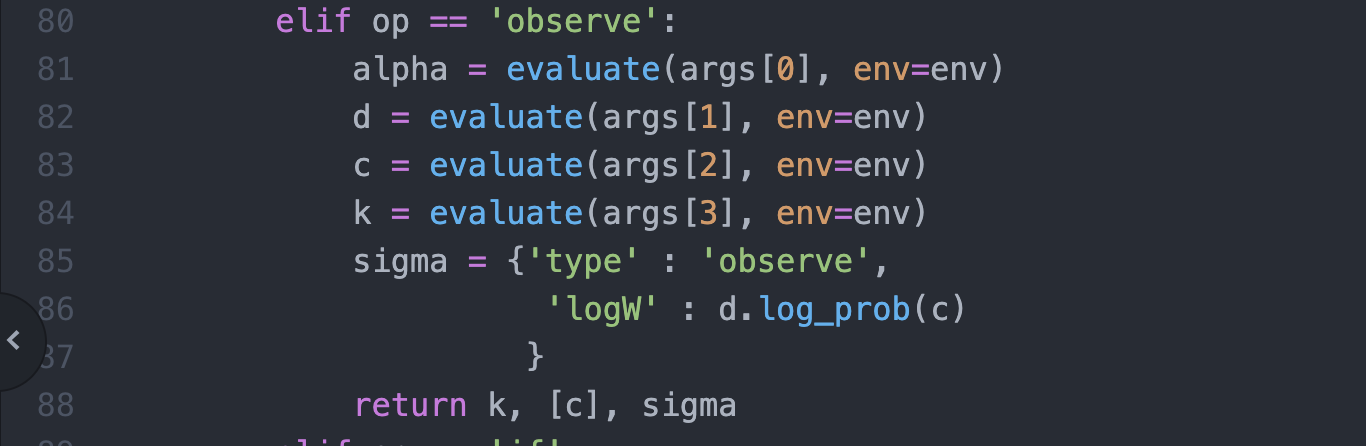
\includegraphics[scale=0.5]{../implementation/observe}
\end{center}

Next, I implemented the resample particles function

\begin{center}
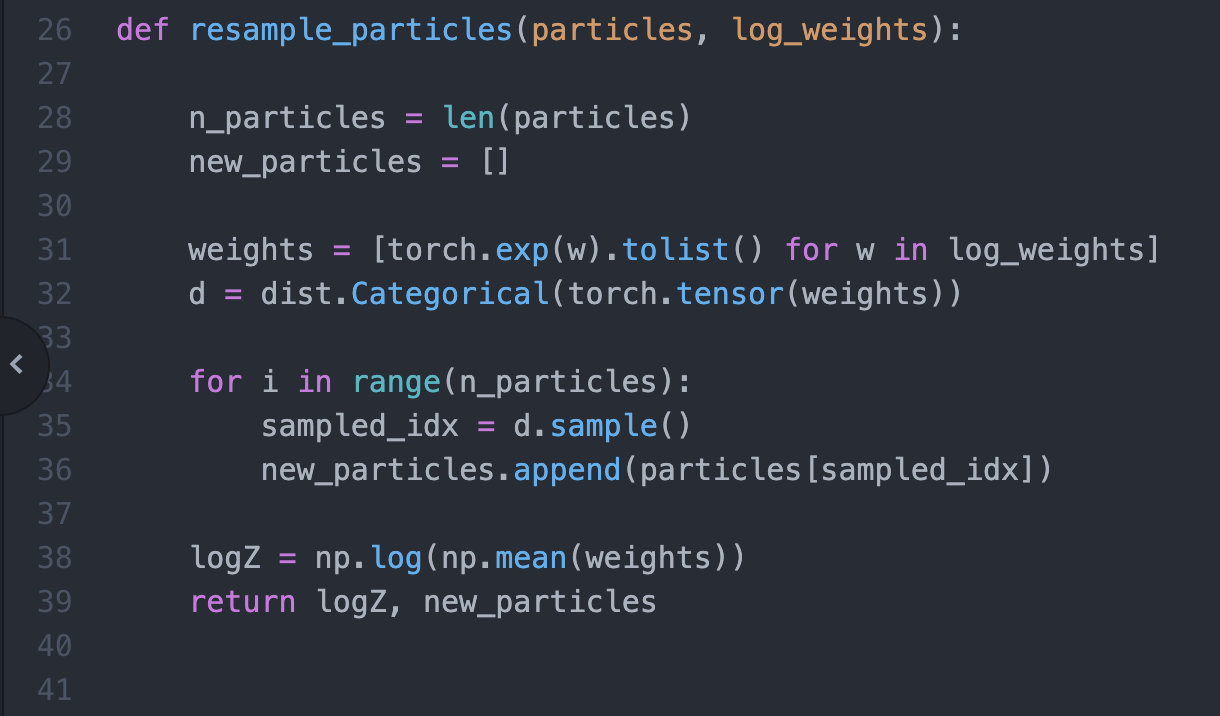
\includegraphics[scale=0.5]{../implementation/resample}
\end{center}

Finally, I implemented the not-done case in the SMC algorithm, extracting the particles and their corresponding weights.

\begin{center}
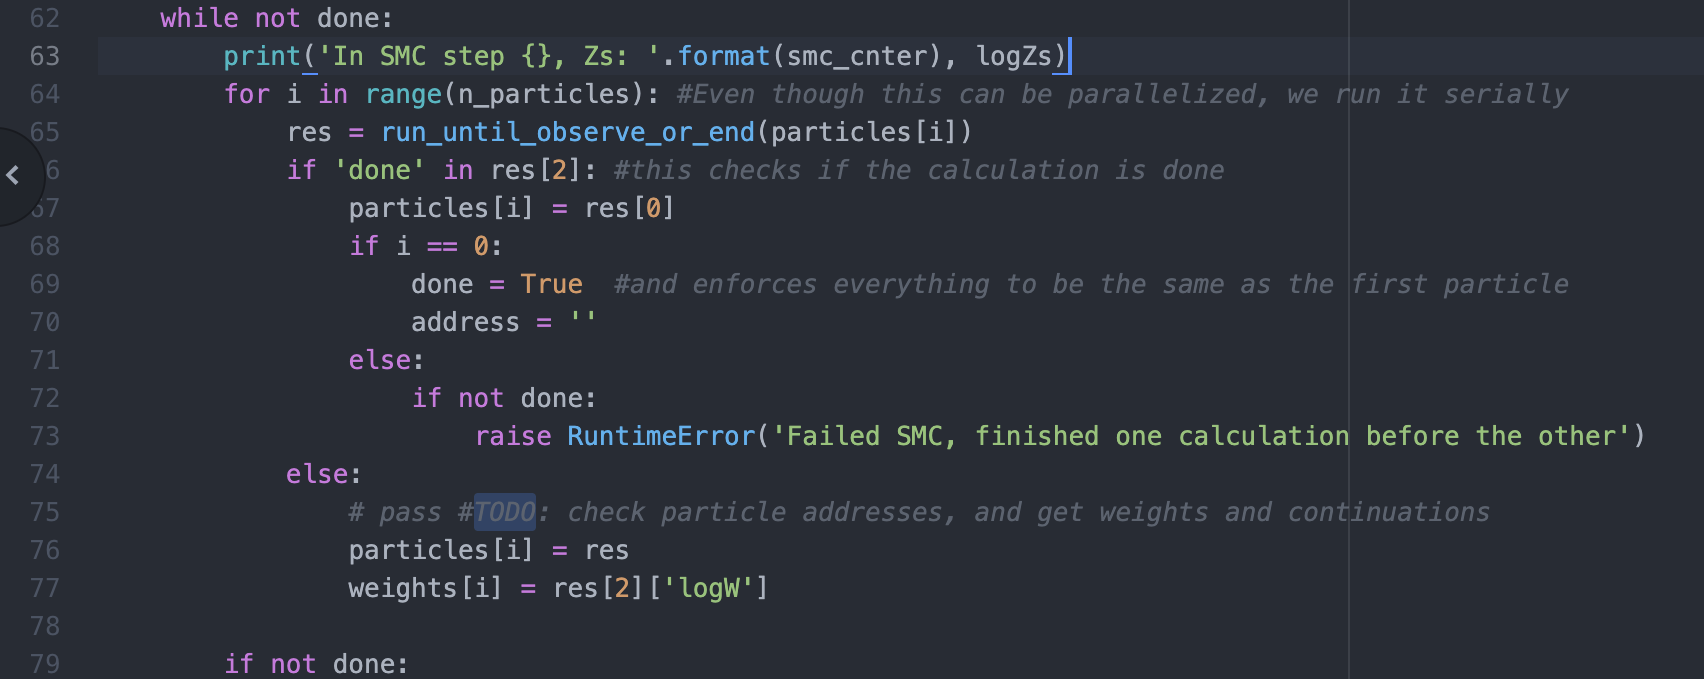
\includegraphics[scale=0.5]{../implementation/return}
\end{center}



\newpage
\section{Program 1}

For program 1 I note that the posterior distribution is equivalent to the prior distribution due to the fact that there are no observe statements in program 1. Consequently, I do not include the evidence estimate for any execution of SMC for program 1 as there are no observed random variables in program 1.

\subsection{1 Particle}

For my execution of SMC for program 1 with a single particle I obtained an estimate of 15.0 for the mean of the posterior. I omit the estimate of the variance of the posterior in this case of a single particle. Below is a histogram for this execution of SMC.

\begin{center}
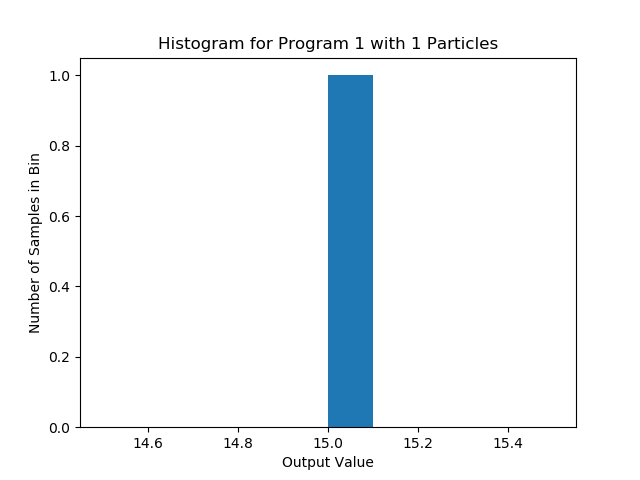
\includegraphics[scale=0.5]{../plots/P1NP1.png}
\end{center}

\subsection{10 Particles}

For my execution of SMC for program 1 with 10 particles I obtained an estimate of 81.0 for the mean of the posterior and an estimate of 4246.6665 for the variance of the posterior. Below is a histogram for this execution of SMC.

\begin{center}
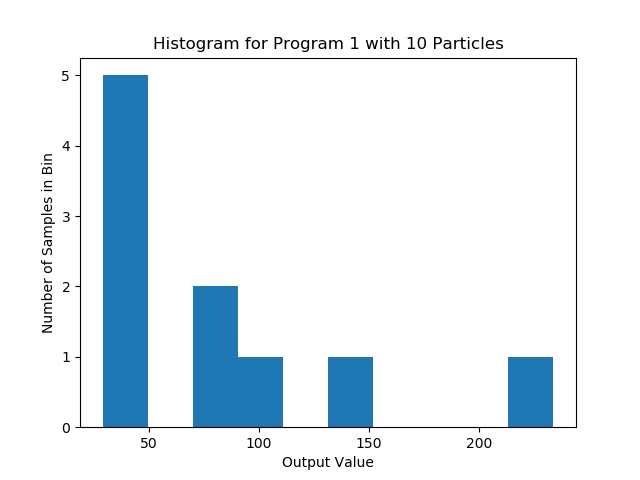
\includegraphics[scale=0.5]{../plots/P1NP10.png}
\end{center}

\subsection{100 Particles}

For my execution of SMC for program 1 with 100 particles I obtained an estimate of 106.87 for the mean of the posterior and an estimate of 14768.6396 for the variance of the posterior. Below is a histogram for this execution of SMC.

\begin{center}
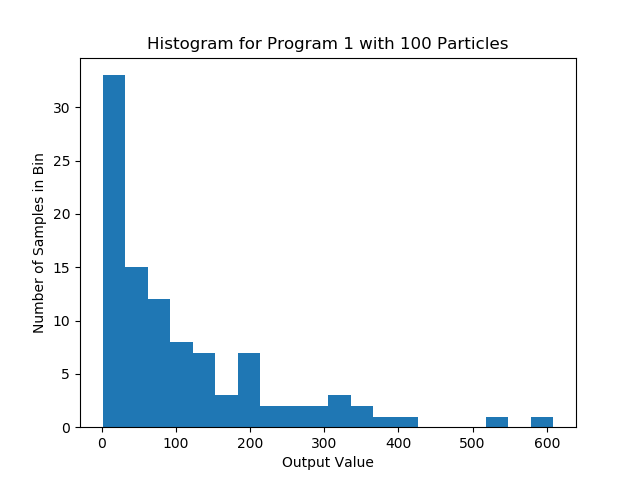
\includegraphics[scale=0.5]{../plots/P1NP100.png}
\end{center}

\subsection{1000 Particles}


For my execution of SMC for program 1 with 1000 particles I obtained an estimate of 100.79499 for the mean of the posterior and an estimate of 10735.7851 for the variance of the posterior. Below is a histogram for this execution of SMC.

\begin{center}
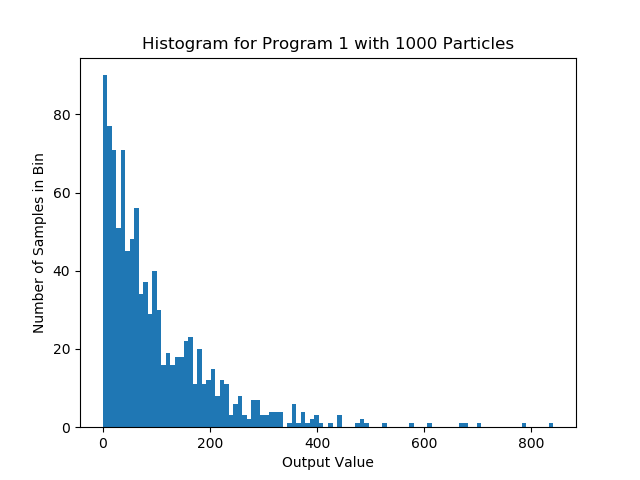
\includegraphics[scale=0.5]{../plots/P1NP1000.png}
\end{center}

\subsection{10000 Particles}

For my execution of SMC for program 1 with 10000 particles I obtained an estimate of 99.2501 for the mean of the posterior and an estimate of 9853.4277 for the variance of the posterior. Below is a histogram for this execution of SMC.

\begin{center}
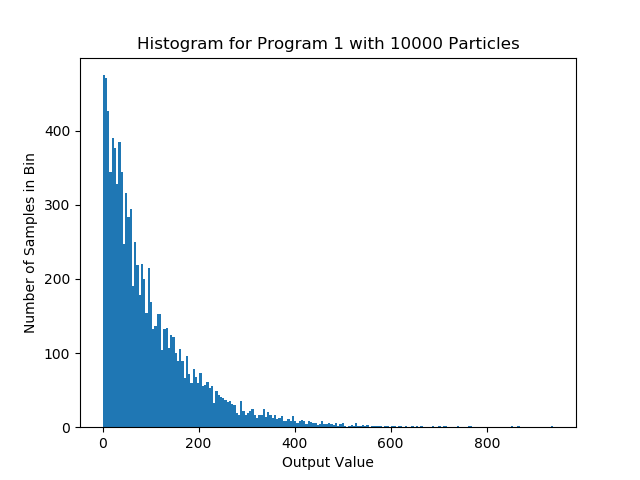
\includegraphics[scale=0.5]{../plots/P1NP10000.png}
\end{center}

\subsection{100000 Particles}

For my execution of SMC for program 1 with 100000 particles I obtained an estimate of 99.7467 for the mean of the posterior and an estimate of  10062.3925 for the variance of the posterior. Below is a histogram for this execution of SMC.

\begin{center}
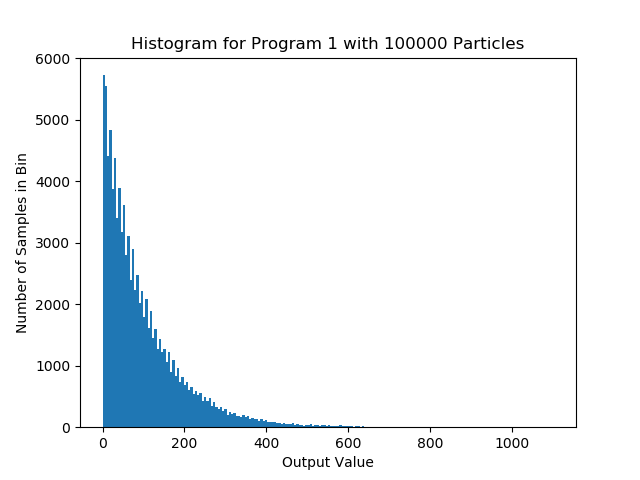
\includegraphics[scale=0.5]{../plots/P1NP100000.png}
\end{center}

\section{Program 2}


\subsection{1 Particle}

For my execution of SMC for program 2 with a single particle I obtained an estimate of 1.8688 for the mean of the posterior and an estimate of -24.6420 for the log evidence. I omit the estimate of the variance of the posterior in this case of a single particle. Below is a histogram for this execution of SMC.

\begin{center}
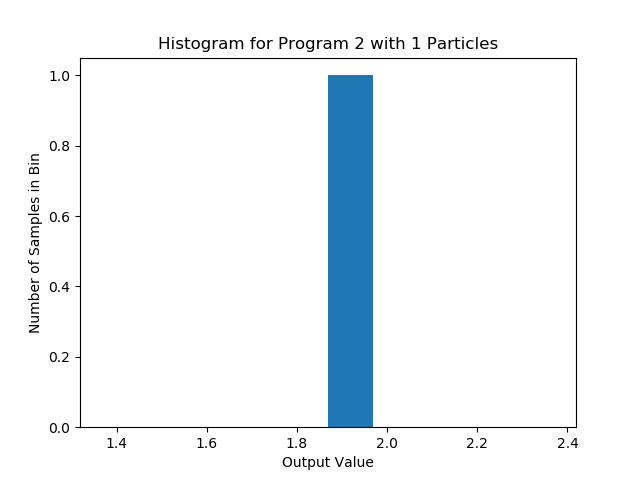
\includegraphics[scale=0.5]{../plots/P2NP1.png}
\end{center}

\subsection{10 Particles}


For my execution of SMC for program 2 with 10000 particles I obtained an estimate of 6.575 for the mean of the posterior, an estimate of 0.0 for the variance of the posterior, and an estimate of -6.8063 for the log evidence. Below is a histogram for this execution of SMC.

\begin{center}
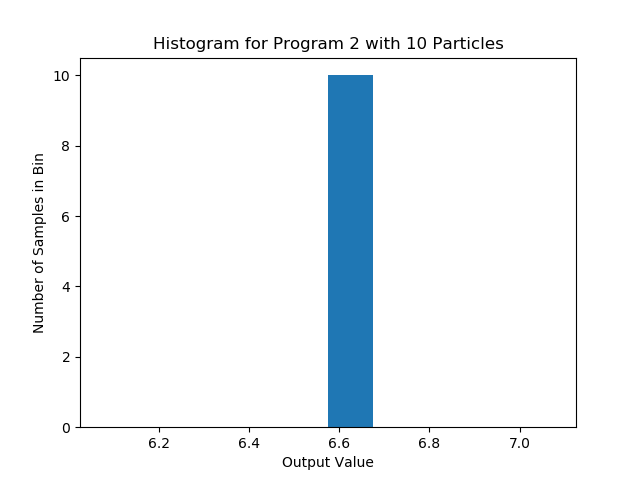
\includegraphics[scale=0.5]{../plots/P2NP10.png}
\end{center}

\subsection{100 Particles}

For my execution of SMC for program 2 with 10000 particles I obtained an estimate of 7.717 for the mean of the posterior, an estimate of 0.0 for the variance of the posterior, and an estimate of -7.7229 for the log evidence. Below is a histogram for this execution of SMC.

\begin{center}
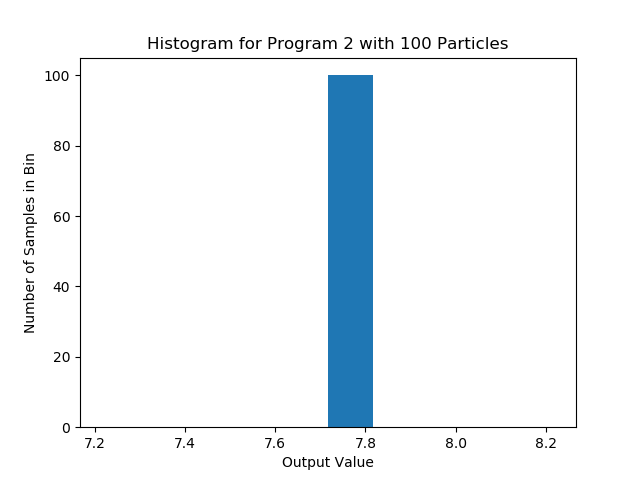
\includegraphics[scale=0.5]{../plots/P2NP100.png}
\end{center}

\subsection{1000 Particles}

For my execution of SMC for program 2 with 10000 particles I obtained an estimate of 7.2853 for the mean of the posterior, an estimate of 0.9801 for the variance of the posterior, and an estimate of -8.2321 for the log evidence. Below is a histogram for this execution of SMC.

\begin{center}
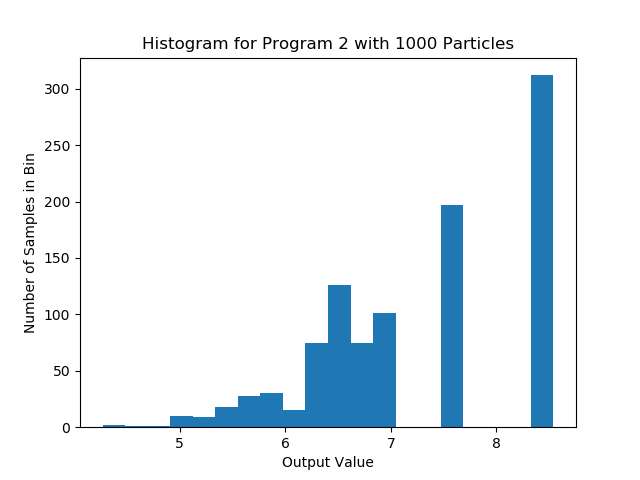
\includegraphics[scale=0.5]{../plots/P2NP1000.png}
\end{center}

\subsection{10000 Particles}

For my execution of SMC for program 2 with 10000 particles I obtained an estimate of 7.2423 for the mean of the posterior, an estimate of 0.85123 for the variance of the posterior, and an estimate of -8.2732 for the log evidence. Below is a histogram for this execution of SMC.

\begin{center}
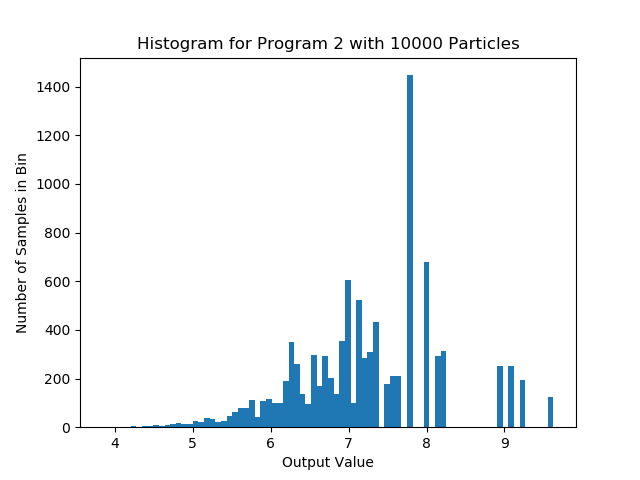
\includegraphics[scale=0.5]{../plots/P2NP10000.png}
\end{center}

\subsection{100000 Particles}

For my execution of SMC for program 2 with 10000 particles I obtained an estimate of 7.2006 for the mean of the posterior, an estimate of 0.82349 for the variance of the posterior, and an estimate of  -8.2674 for the log evidence. Below is a histogram for this execution of SMC.

\begin{center}
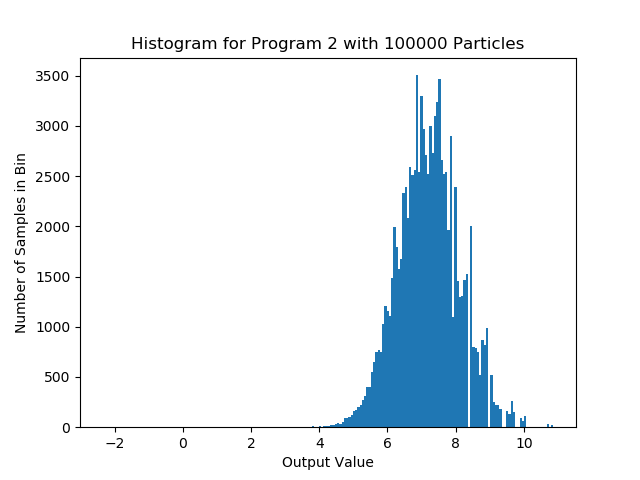
\includegraphics[scale=0.5]{../plots/P2NP100000.png}
\end{center}

\section{Program 3}

Note, my means and variances for program 3 are presented as a vector ordered from time step 1 to time step 17.

\subsection{1 Particle}

For my execution of SMC for program 3 with a single particle I obtained the following estimate of the mean of the posterior:

[1., 2., 2., 2., 2., 2., 2., 2., 0., 1., 0., 2., 2., 2., 1., 2., 1.] 

I omit the estimate of the variance of the posterior due to the use of a single particle. I obtained the following estimate of the log evidence: -48.953. Below is a histogram for this execution of SMC.

\begin{center}
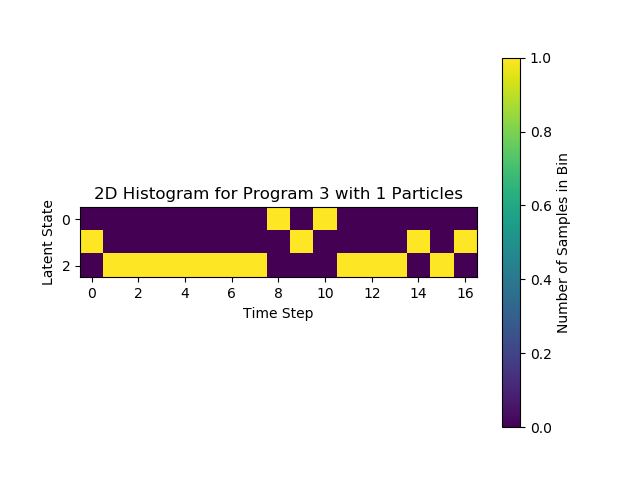
\includegraphics[scale=0.5]{../plots/P3NP1.png}
\end{center}

\subsection{10 Particles}


For my execution of SMC for program 3 with a 10 particles I obtained the following estimate of the mean of the posterior:

[2., 1.8, 2., 2., 1., 2., 2., 2., 1., 0., 0., 2., 2., 2., 2., 2., 0.]

I obtained the following estimate of the variance of the posterior:

[0., 0.4, 0., 0., 0., 0., 0., 0., 0., 0., 0., 0., 0., 0., 0., 0., 0.]

I obtained the following estimate of the log evidence: -44.3966. Below is a histogram for this execution of SMC.

\begin{center}
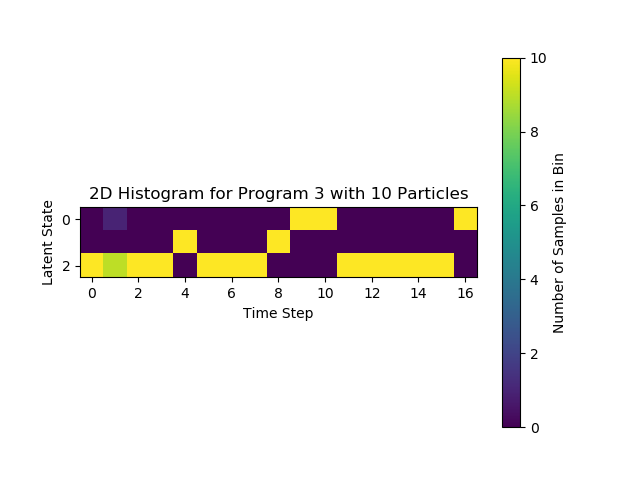
\includegraphics[scale=0.5]{../plots/P3NP10.png}
\end{center}

\subsection{100 Particles}

For my execution of SMC for program 3 with a 100 particles I obtained the following estimate of the mean of the posterior:

[1.39, 1.52, 1.9, 1.61, 1.05, 1.51, 1.66, 1.55, 1.9, 0.62, 0.06, 2., 1.64, 1.78, 1.59, 1.52, 1.48]

I obtained the following estimate of the variance of the posterior:

[0.8060, 0.6158, 0.1111, 0.4423, 0.0480, 0.4342, 0.5095, 0.6136, 0.0909, 0.8440, 0.1176, 0.0, 0.5156, 0.1733, 0.4666, 0.3733, 0.6158]

I obtained the following estimate of the log evidence: -44.2297. Below is a histogram for this execution of SMC.

\begin{center}
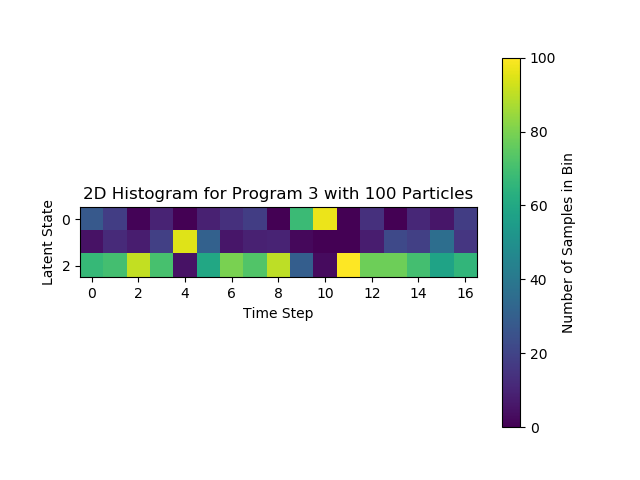
\includegraphics[scale=0.5]{../plots/P3NP100.png}
\end{center}

\subsection{1000 Particles}


For my execution of SMC for program 3 with a 1000 particles I obtained the following estimate of the mean of the posterior:

[1.381, 1.582, 1.746, 1.643, 1.025, 1.437, 1.586, 1.495, 1.463, 0.9480, 0.1120, 1.7300, 1.653, 1.696, 1.708, 1.61, 1.113]

I obtained the following estimate of the variance of the posterior:

[0.7926, 0.6159, 0.2778, 0.4400, 0.0244, 0.6146, 0.433, 0.5625, 0.5792,0.9683, 0.2117, 0.3515, 0.4871, 0.2739, 0.249, 0.3282, 0.6469]

I obtained the following estimate of the log evidence: -44.3568. Below is a histogram for this execution of SMC.

\begin{center}
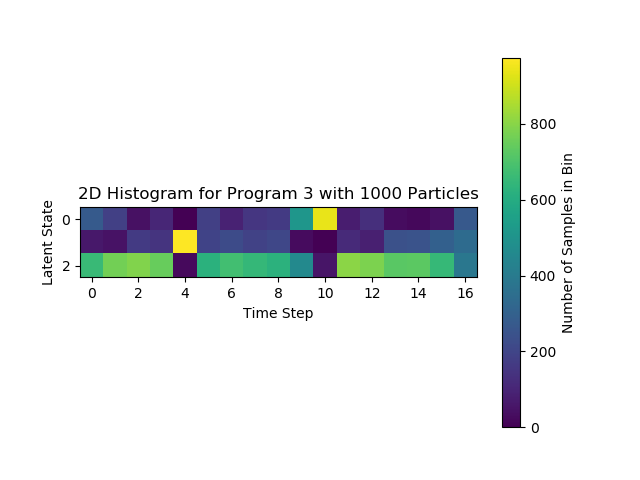
\includegraphics[scale=0.5]{../plots/P3NP1000.png}
\end{center}

\subsection{10000 Particles}

For my execution of SMC for program 3 with a 10000 particles I obtained the following estimate of the mean of the posterior:

[1.4168, 1.5557, 1.6935, 1.6121, 1.0157, 1.4365, 1.6653, 1.6493, 1.6108, 1.0968, 0.1392, 1.7129, 1.6679, 1.6603, 1.6883, 1.4934, 0.9226]

I obtained the following estimate of the variance of the posterior:

[0.7600, 0.6412, 0.3292, 0.4709, 0.0155, 0.5878, 0.4065, 0.4326, 0.4098, 0.9579, 0.2590, 0.3269, 0.4349, 0.3175, 0.3098, 0.3668, 0.7025]

I obtained the following estimate of the log evidence:  -44.3738. Below is a histogram for this execution of SMC.

\begin{center}
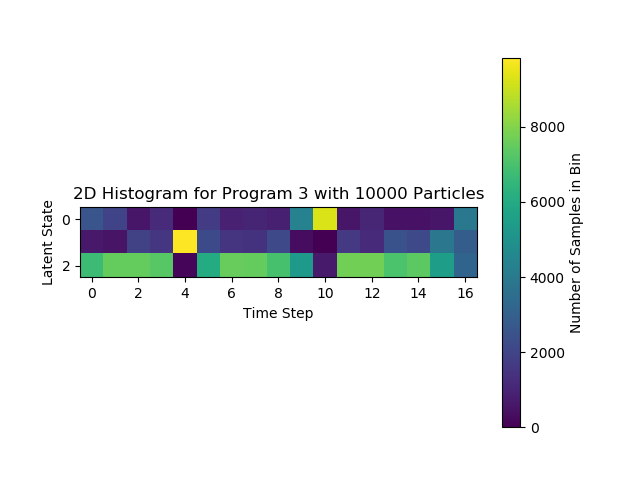
\includegraphics[scale=0.5]{../plots/P3NP10000.png}
\end{center}

\subsection{100000 Particles}


For my execution of SMC for program 3 with a 100000 particles I obtained the following estimate of the mean of the posterior:

[1.4294, 1.5484, 1.6994, 1.5994, 1.0160, 1.4274, 1.6419, 1.6588, 1.6012, 1.0775, 0.1452, 1.6971, 1.6549, 1.6806, 1.6220, 1.5047, 0.9164]

I obtained the following estimate of the variance of the posterior:

[0.7549, 0.6526, 0.3249, 0.4719, 0.0180, 0.5958, 0.4315, 0.4238, 0.4245, 0.9510, 0.2642, 0.3421, 0.4476, 0.3124, 0.3457, 0.3225, 0.6870]

I obtained the following estimate of the log evidence:  -44.41369. Below is a histogram for this execution of SMC.

\begin{center}
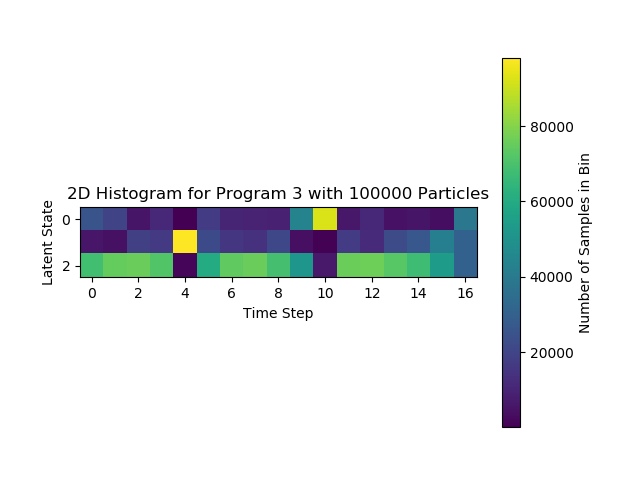
\includegraphics[scale=0.5]{../plots/P3NP100000.png}
\end{center}

\end{document}
